\section{CCP Implementation}
\label{s:datapath}
%
\begin{figure}[t]
\centering
    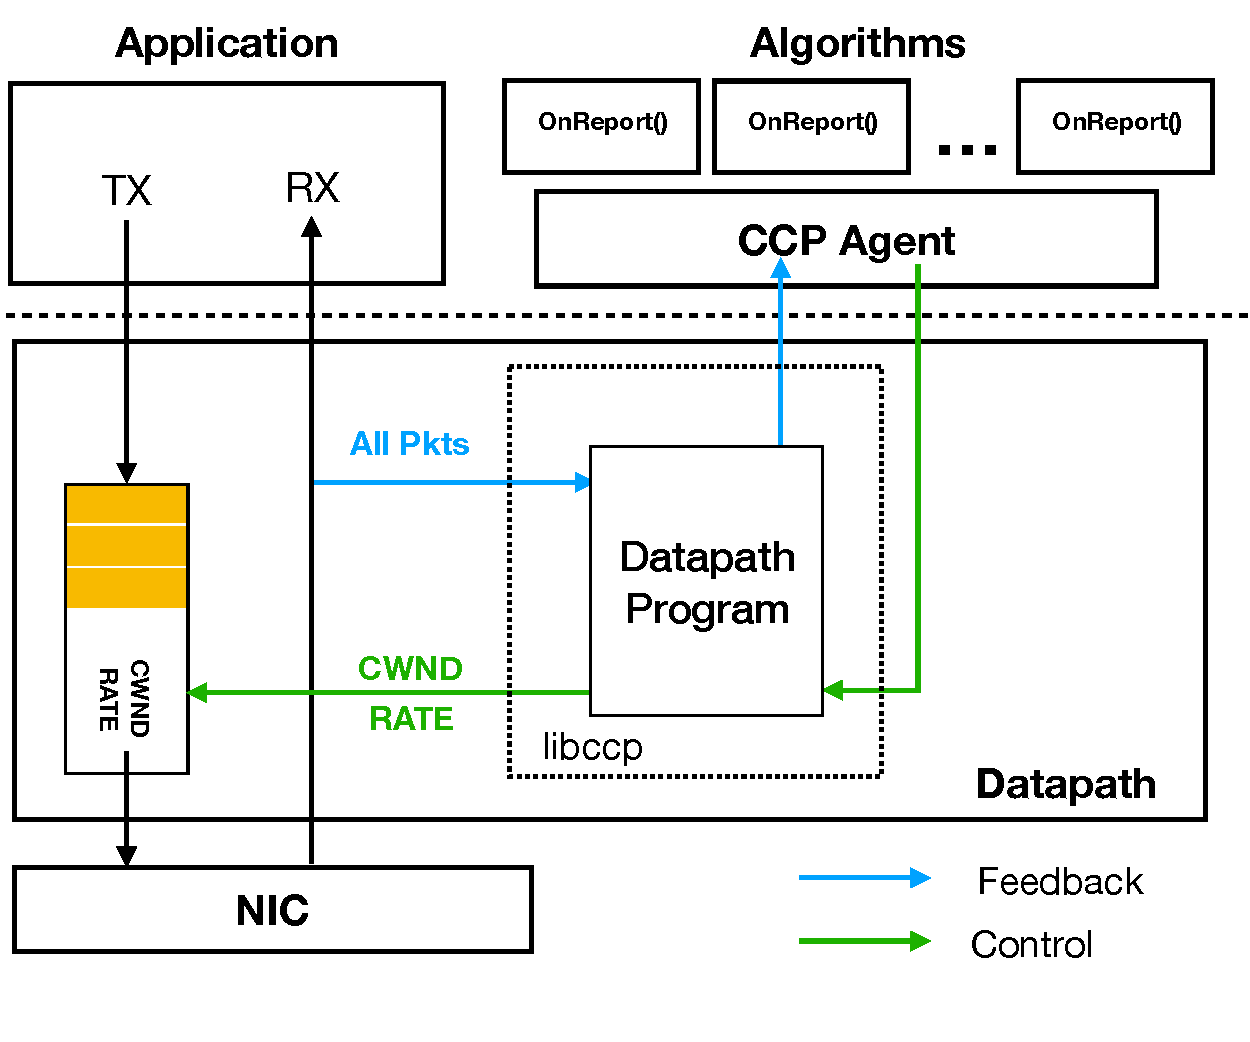
\includegraphics[width=\columnwidth]{img/ccp_design_sigcomm}
    \caption{Congestion control algorithms in CCP are distinct from both the application and datapath. Algorithm implementations are split between a slow path in user-space and a fast path embedded in the datapath.}\label{fig:design}
\end{figure}
%
Figure~\ref{fig:design} summarizes the architecture of a CCP-enabled sender,
highlighting how the various components interact.

\subsection{CCP Design Principles}
\label{s:datapath:isolation}

To enable rich new congestion control algorithms on the Linux networking stack,
CCP must provide a low-barrier programming environment and access
to libraries (\eg for optimization, machine learning, \etc).
%
Further, new algorithms should also achieve high performance running at tens of
Gbit/s per connection with small ``in-stack'' packet delays.

However, supporting experimentation and libraries (typically
\userspace code) means that congestion control algorithm code is untrusted.
Otherwise, bugs in algorithm or library code could cause kernel
crashes or create vulnerabilities that could trigger privilege escalation
attacks on the kernel.

\Para{Explicit fast and slow path separation.} While algorithms must have
some component running in the same address space as the kernel to collect measurements,
we restrict this functionality by requiring {\em explicit fast and slow path} components for algorithms:
the fast path runs in the Linux kernel, and the slow path in \userspace.
%
An alternative, which is to allow fully functional kernel modules with software
fault isolation (\eg LXFI~\cite{lxfi}) from the rest of the kernel, will likely
involve significant performance impediments.\footnote{Further, an approach such as
LXFI also requires a careful annotation of kernel functions, and the
specification of principals and kernel API integrity rules---a challenging
task because the network stack has a large number of functions with subtle
behaviors.}
%
Instead, our fast path programs are written in a restrictive domain-specific language (\Sec{sec:ccp})
that is free from broad classes of vulnerabilities.\footnote{Note that while \texttt{libccp}, our fast path library (\Sec{s:datapath:libccp}), enforces runtime safety of fast-path algorithm logic,
algorithm implementations are nevertheless free to set arbitrary rates or congestion windows.
As any application can open UDP sockets and congest the network, we do not restrict this behavior.}
Meanwhile, slow path programs have full access to the \userspace programming environment,
tools, and libraries.

Explicit fast and slow path separation also enables future use cases where the
slow paths of algorithms may run on a machine different from the sender to
centralize congestion control policies across groups of hosts.

\begin{table}[]
    \centering
    \begin{tabular}{c|c|c}
        Implementation & Reporting Interval & Mean Throughput \\
        \hline
        Kernel & - & $43$ Gbit/s \\
        CCP & Per ACK & $29$ Gbit/s \\
        CCP & Per $10$ ms & $41$ Gbit/s \\
    \end{tabular}
    \caption{Single-flow throughput for different reporting intervals between
      the Linux kernel and CCP \userspace, compared to kernel TCP
      throughput. Per-ACK feedback (0 $\mu$s interval) reduces throughput by
      32\% while using a $10$ ms reporting interval
      achieves almost identical throughput to the kernel. Results as the number
      of flows  increases are in
      \S\ref{sec:eval:whyfold}.}\label{tab:perf:interval}
\end{table}

\Para{Decoupling algorithm logic from the ACK clock.} Typical congestion control
implementations in the Linux kernel are coupled to the so-called ``ACK-clock,''
\ie algorithm functionality is invoked upon receiving a packet acknowledgment in
the networking stack.
%
While this is also true of a CCP algorithm's fast path, the CCP slow path is
only invoked when the user specifies, whether less frequently than per-ACK or in response to certain urgent conditions.
%
To support this, CCP exposes a \ct{report} instruction for fast path programs to send a
report of the most recent user-defined measurement state in the kernel to the slow path.

This decoupling of algorithm logic from the ACK clock has two benefits.
%
First, the user can develop congestion control algorithms free from the strict
time restrictions rooted in the inter-arrival time of packet acknowledgments,
especially at high link rates.
Hence, users can implement algorithms that use complex logic and yet retain high performance.

Second, providing per-ACK notifications from the kernel to \userspace would incur
significant overhead.
%
Table~\ref{tab:perf:interval} shows that for a single saturating \ct{iperf}
connection over a loopback interface, Linux kernel TCP on a server machine
with four 2.8-Ghz cores achieves $45$ Gbit/s running Reno.
%
In comparison, per-ACK reporting from the kernel to the CCP \userspace achieves
only 68\% of the kernel's throughput.
%
By increasing the time between reports sent to the slow path to 10 ms (see the
``per 10 ms'' row), CCP Reno achieves close to the kernel's throughput.

Given that CCP should report measurements only infrequently, a key question is
how best to summarize congestion signals within the fast path, so that CCP
algorithms can achieve high fidelity compared to a baseline that implements the
algorithm completely within the kernel.
Although we are optimistic that a good design can achieve high fidelity because the natural time-scale for end-to-end
congestion control is the RTT between sender and receiver,
achieving it requires a careful design of the information channel between the kernel and CCP \userspace.
Indeed, in \S\ref{sec:eval:fidelity} we show that using a
larger reporting period does not affect the fidelity of CCP algorithm
implementations relative to native in-kernel implementations.

\subsection{Overview of the Linux fast path implementation}
\label{sec:implementation-basics}

An implementation of the CCP fast path must perform the following functions:
\begin{itemize}
\item The fast path should communicate with a \userspace CCP agent using an IPC
  mechanism. The fast path multiplexes \ct{report}s from multiple connections
  onto the single persistent IPC connection to the slow path.
\item The fast path should execute the user-provided domain-specific program on
  the arrival of every acknowledgment or a timeout in a safe manner. Fast path
  programs (\Sec{sec:ccp}) may include simple computations to summarize
  per-packet congestion signals (Table~\ref{tab:api}) and enforce congestion
  windows and rates.
\end{itemize}

We have implemented a Linux kernel fast path as a kernel
module over the Linux 4.14 kernel. The module
implements the communication channel to the slow path using either netlink sockets or a custom
character device.

Our kernel module leverages the pluggable TCP API to invoke the program
interpreter upon arrivals of packet acknowledgments and timeouts.
%
\begin{table}
    \centering
    \footnotesize
    \begin{tabular}{p{0.35\columnwidth}p{0.5\columnwidth}}
        \textbf{Signal} & \textbf{Definition} \\
        \hline
        \texttt{Ack.bytes\_acked}, \texttt{Ack.packets\_acked}             & \texttt{Delta(tcp\_sock.bytes\_acked)} \\
        \texttt{Ack.bytes\_misordered}, \texttt{Ack.packets\_misordered}   & \texttt{Delta(tcp\_sock.sacked\_out)} \\
        \texttt{Ack.ecn\_bytes}, \texttt{Ack.ecn\_packets}                 & \texttt{in\_ack\_event: CA\_ACK\_ECE} \\
        \texttt{Ack.lost\_pkts\_sample}                                    & \texttt{rate\_sample.losses} \\
        \texttt{Ack.now}                                                   & \texttt{getnstimeofday()}\\
        \texttt{Flow.was\_timeout}                                         & \texttt{set\_state: TCP\_CA\_Loss} \\
        \texttt{Flow.rtt\_sample\_us}                                      & \texttt{rate\_sample.rtt\_us} \\
        \texttt{Flow.rate\_outgoing}                                       & \texttt{rate\_sample.delivered / Delta(tcp\_sock.first\_tx\_mstamp)} \\
        \texttt{Flow.rate\_incoming}                                       & \texttt{rate\_sample.delivered / Delta(tcp\_sock.tcp\_mstamp)}  \\
        \texttt{Flow.bytes\_in\_flight}, \texttt{Flow.packets\_in\_flight} & \texttt{tcp\_packets\_in\_flight(tcp\_sock)} \\
    \end{tabular}
    %\vspace{0.075in}
    \caption{Definition of CCP primitives in terms of \texttt{tcp\_sock} state.}\label{tab:api:kernel}
\end{table}
Our implementation extracts primitive congestion signals from the
\ct{tcp\_sock} and \ct{rate\_sample} structures.

Table ~\ref{tab:api:kernel} details the mapping of kernel variables
to CCP primitives.
%
The module enforces congestion windows and sending rates using the corresponding
members of the \ct{tcp\_sock} and \ct{sock} structures (\ct{snd\_cwnd} and
\ct{sk\_pacing\_rate}, respectively).

This definition of primitives and enforcement mechanisms is the only datapath-specific
work needed to support CCP; all other functionality is shared amongst software datapaths
via the program interpreter: \texttt{libccp}. In addition to Linux, we have already integrated
\ct{libccp} into CCP fast path implementations running inside Intel DPDK and
QUIC.


\subsection{Safe Execution of fast path programs}
\label{s:datapath:fold}
Datapaths are responsible for safely executing the fast path program sent from the userspace CCP module. While CCP will serialize the instructions and check for mundane errors (e.g., use of undefined variables) before installation, it is the datapath’s responsibility to ensure safe interpretation of the instructions. For example, datapaths should prevent divide by zero errors when calculating user defined variables and guarantee that programs cannot overwrite the congestion primitives.

Thankfully, this task is straightforward as fast path programs are limited in functionality.
Programs may not enter loops, perform floating point operations, define functions or data structures, allocate memory, or access arbitrary memory addresses; programs are strictly a way to express arithmetic computations over a limited set of primitives, define when and how to set congestion windows and pacing rates, and report measurements.

We have implemented a library, \ct{libccp}, that provides a reference
implementation of CCP's datapath component; \ie an execution environment for
user-specified datapath behavior and message serialization for software
datapaths. While we considered using eBPF~\cite{ebpf} or TCP BPF~\cite{tcpbpf}
for this functionality, using our own lightweight virtual machine, \ct{libccp},
allowed us to port our CCP implementations to other datapaths outside the
kernel, such as QUIC, with minimal effort.

\subsection{\ct{libccp}: a fast path program interpreter}
\label{s:datapath:libccp}
To use \ct{libccp}, the datapath must provide callbacks to functions that: (1) set the window and rate, (2) provide a notion of time, and (3) send an IPC message to CCP. Upon read- ing a message from CCP, the datapath calls \ct{ccp\_recv\_msg()}, which automatically demultiplexes the message for the correct flow. After updating congestion signals, the datapath can call \ct{ccp\_invoke()}, which automatically runs the fastpath program, which may update variable calculations, set windows or rates, and send report summaries to the CCP. It is the responsibility of the datapath to ensure that it correctly computes and provides the congestion signals in Table 1.
The more signals a datapath can measure, the more algorithms that datapath can support. For example, CCP can only support DCTCP \cite{DCTCP} or ABC \cite{abc} on datapaths that provide ECN support; CCP will not run algorithms on datapaths lacking support for that algorithm’s requisite primitives.
